\documentclass{llncs}

\usepackage{llncsdoc}
\usepackage{multirow}
\usepackage{verbatim}

\usepackage{tikz}
\usepackage{pgfplots}
\pgfplotsset{compat=1.10}
\usetikzlibrary{shapes.geometric,arrows,fit,matrix,positioning,pgfplots.groupplots}
\usepackage{circuitikz}
\usepackage{comment}
\usepackage[ruled,vlined,linesnumbered,noresetcount]{algorithm2e}
\AlgoDisplayBlockMarkers 
\SetAlFnt{\footnotesize}
%\SetAlFnt{\small}
\usepackage{setspace}

\tikzset
{
    treenode/.style = {circle, draw=black, align=center, minimum size=1cm},
    subtree/.style  = {isosceles triangle, draw=black, align=center, minimum height=0.5cm, minimum width=1cm, shape border rotate=90, anchor=north}
}

%macros
\newcommand{\node}{\textit{node}}
\newcommand{\terminalnode}{\textit{terminal node}}
\newcommand{\readyToReplace}{\textit{readyToReplace}}
\newcommand{\markAndKey}{\textit{markAndKey}}
\newcommand{\child}{\textit{child}}
\newcommand{\deleteFlag}{\textit{deleteFlag}}
\newcommand{\promoteFlag}{\textit{promoteFlag}}
\newcommand{\nullFlag}{\textit{nullFlag}}
\newcommand{\anchorNode}{\textit{anchor node}}
\newcommand{\parent}{\textit{parent}}
\newcommand{\lastUParent}{\textit{lastUParent}}
\newcommand{\lastUNode}{\textit{lastUNode}}
\newcommand{\injectionPoint}{\textit{injectionPoint}}
\newcommand{\mode}{\textit{mode}}
\newcommand{\type}{\textit{type}}
\newcommand{\seekRecord}{\textit{seekRec}}
\newcommand{\mySeekRecord}{\textit{mySeekRec}}
\newcommand{\succNode}{\textit{succNode}}
\newcommand{\succParent}{\textit{succParent}}
\newcommand{\state}{\textit{state}}
\newcommand{\myState}{\textit{myState}}
\newcommand{\lastRNode}{\textit{anchor node}}
\newcommand{\lastRKey}{\textit{anchor key}}
\newcommand{\cSeek}{\textit{cSeek}}
\newcommand{\pSeek}{\textit{pSeek}}
\newcommand{\cKey}{\textit{cKey}}
\newcommand{\nKey}{\textit{nKey}}
\newcommand{\pKey}{\textit{pKey}}
\newcommand{\which}{\textit{which}}
\newcommand{\pWhich}{\textit{pWhich}}
\newcommand{\nWhich}{\textit{nWhich}}
\newcommand{\address}{\textit{address}}
\newcommand{\result}{\textit{out}}
\newcommand{\newNode}{\textit{newNode}}
\newcommand{\needToHelp}{\textit{needToHelp}}
\newcommand{\Left}{\textit{left}}
\newcommand{\Right}{\textit{right}}
\newcommand{\key}{\textit{key}}
\newcommand{\lN}{\textit{lN}}
\newcommand{\rN}{\textit{rN}}
\newcommand{\prev}{\textit{prev}}
\newcommand{\curr}{\textit{curr}}
\newcommand{\dFlag}{\textit{dFlg}}
\newcommand{\done}{\textit{done}}
\newcommand{\accesspath}{\textit{access-path}}
\newcommand{\return}{\textbf{return}}
\newcommand{\Break}{\textbf{break}}
\newcommand{\True}{\textit{true}}
\newcommand{\False}{\textit{false}}

\begin{document}
\title{A Fast Lock-Free Internal Binary Search Tree}

\author{Arunmoezhi Ramachandran, Neeraj Mittal}

\institute{Department of Computer Science, The University of Texas at Dallas, Richardson, Texas 75080, USA \\ \email{(arunmoezhi,neerajm)@utdallas.edu}}

\maketitle

\begin{abstract}
We present a new \textit{lock-free} algorithm for concurrent manipulation of a binary search tree in an asynchronous shared memory system that supports search, insert and delete operations. Our algorithm uses (single-word) compare-and-swap (CAS) and bit-test-and-set (BTS) atomic instructions, both of which are commonly supported by many modern processors including Intel 64 and AMD64. We minimize conflicts by marking \textit{edges} rather than \textit{nodes}. We also reduce memory footprint by a factor of 2 by using an internal representation of a binary search tree. Compared to existing \textit{lock-free} algorithms, our algorithm uses fewer atomic instructions in the absence of conflicts. Our experiments indicate that our \textit{lock-free} algorithm significantly outperforms all other algorithms for a concurrent binary search tree in many cases, by as much as 70$\%$.
\end{abstract}

\keywords
Concurrent Data Structure, Lock-Free Algorithm, Binary Search Tree

\section{Introduction}
A Binary Search Tree (BST) implements the dictionary abstract data type. In a BST, all the values in a node's left subtree are less than the node value and all the values in the node's right subtree are greater than the node value. Duplicates are not allowed. A BST supports three main operations, viz.: search, insert and delete. Search($x$) determines if $x$ is present in the tree. Insert($x$) adds key $x$ to the tree if it is not already present. Delete($x$) removes the key $x$ from the tree if it is present. \par
Several algorithms have been proposed for non-blocking binary search trees. Ellen \textit{et al.} proposed the first practical lock-free algorithm for a concurrent binary search tree in~\cite{EllFat+:2010:PODC}. Their algorithm uses an external (or leaf-oriented) search tree in which only the leaf nodes store the actual keys; keys stored at internal nodes are used for routing purposes only. Howley and Jones have proposed another lock-free algorithm for a concurrent binary search tree in~\cite{HowJon:2012:SPAA} which uses an internal search tree in which both the leaf nodes as well as the internal nodes store the actual keys. One advantage of using an internal search tree is that its memory footprint is half that of an external search tree. For large size trees, search time dominates and our experimental results shows that internal BST tend to perform better than external BSTs. Natarajan and Mittal have proposed another lock-free external BST in~\cite{Natarajan:2014:PPOPP}. The key change in this algorithm is that it operates at edge level and the ones described by Ellen \textit{et al.}~\cite{EllFat+:2010:PODC} and Howley and Jones~\cite{HowJon:2012:SPAA}  operates on node level. A node (or edge) level operation mean that nodes (or edges) are marked for deletion. Operating at edge level blocks fewer operations than operating at node level. So edge level operation provides more concurrency when there is high contention. Hence the algorithm described by Natarajan and Mittal~\cite{Natarajan:2014:PPOPP} performs well for smaller trees with high contention. We have designed our algorithm to get the benefits of both the worlds. Our algorithm like the one proposed by Howley and Jones~\cite{HowJon:2012:SPAA} is an internal BST and like the one proposed by Natarajan and Mittal~\cite{Natarajan:2014:PPOPP} operate on edge level.

\input{model}

\section{Lock-Free Algorithm}
\subsection{Overview}
Every operation in our algorithm begins with a seek phase. 
\subsubsection{Seek:} The operation traverses the search tree from the root node until it finds the target key or if it reaches a non-binary node. We refer to the path traversed by the operation in the seek phase as the \accesspath \space and the last node in the \accesspath \space is referred to as \terminalnode. The operation then compares the target key with the value stored in the \terminalnode. Depending on the result of the comparison and the type of the operation, the operation either terminates or moves to the next phase. In certain cases in which a key may have moved upward along the \accesspath, the seek operation may have to restart (will be discussed later). We now describe the next steps for each of the type of operation one-by-one.
\subsubsection{Search:} A search operation invokes seek and returns \True \space if the stored key matches the target key; otherwise it returns \False.
\subsubsection{Insert:} An insert operation invokes seek and returns \False \space if the key in the \terminalnode \space matches the target key; otherwise it moves to the execution phase. In the execution phase, it attempts to insert the key into the tree as a child node of the last node in the \accesspath \space using a CAS instruction. If the instruction succeeds, then the operation returns \True; otherwise, it restarts from the seek phase after possibly helping.
\subsubsection{Delete:} A delete operation invokes seek and returns \False \space if the stored key does not match the target key; otherwise it moves to the execution phase. In the execution phase, it attempts to remove the key stored in the \terminalnode \space of the \accesspath. There are two cases depending on if the \terminalnode \space is a binary node (has two children) or not (at most one child). In the first case, the operation is referred to as \textit{complex} delete. In the second case, it is referred to as \textit{simple} delete. In the case of \textit{simple} delete (as shown in Fig.~\ref{fig:simple}), the \terminalnode \space is removed by changing the pointer at the parent of the \terminalnode. In the case of \textit{complex} delete (as shown in Fig.~\ref{fig:complex}), the key to be deleted is replaced with the next largest key in the tree (which will be stored in the leftmost node of the right subtree of the \terminalnode). 

\subsection{Details of the Algorithm}
\input{pseudocode/structures}
We use sentinel keys and nodes to handle the boundary cases easily. A tree node in our algorithm consists of three fields: (i) \markAndKey \space which contains the key stored in the node, (ii) \child \space array, which contains the addresses of the left and right children and (iii) \readyToReplace, which is a boolean flag used by \textit{complex} delete operation to indicate if a node can be replaced with a fresh copy of it. \par
This algorithm like the algorithm described by Natarajan and Mittal~\cite{Natarajan:2014:PPOPP}, operates on edge level. A delete operation obtains ownership of the edges it needs to work on by marking them. To enable marking we steal two bits from the child addresses of a node. To avoid ABA problem, as in Howley and Jones~\cite{HowJon:2012:SPAA}, we steal another bit from the child address referred to as \nullFlag \space and use it to indicate whether the address points to a null or a non-null value. So when an address changes from a non-null value to a null value, we only set the \nullFlag \space and the contents of the address are not modified. As \textit{complex} delete replaces a key in a node being deleted, a flag is required to identify if the key in a node has changed. So we steal a bit from the key field and use it as a mark bit. If the mark bit is set, it denotes that the key in the node has changed.

We next describe the details of the seek phase, which is executed by all operations (search as well as modify) after which we describe the details of the execution phases of insert and delete operations.

\subsubsection{The Seek Phase} \paragraph{}
\begin{figure}
\begin{minipage}[t]{.4\textwidth}
\caption{Sentinel nodes and keys ($\infty$$_0$ $<$ $\infty$$_1$) \label{fig:sentinel}}
{
	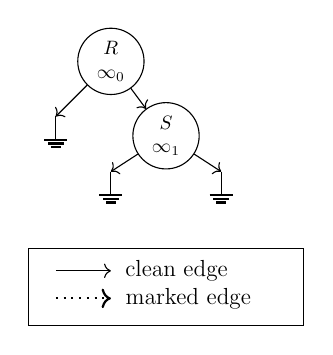
\begin{tikzpicture}[scale=0.7, transform shape]
	\newcommand\XA{0}
\newcommand\YA{0}
\newcommand\XB{\XA-1}
\newcommand\YB{\YA-3.8}
\node (R)			[treenode] 									at (\XA,\YA)       	{$R$ \\ $\infty$$_0$};
\node (gnd)		[ground] 										at (\XA-1,\YA-1)			{}; 
\node (S)			[treenode] 									at (\XA+1,\YA-1.35) 		{$S$ \\ $\infty$$_1$};
\node (gndls)	[ground] 										at (\XA,\YA-2)				{}; 
\node (gndrs)	[ground] 										at (\XA+2,\YA-2)				{}; 


\path[every node/.style={font=\sffamily\small}]
(R) 		edge[->] 								node  				{} (S)
(R) 		edge[->] 								node 				 	{} (gnd)
(S) edge[->] node {} (gndls)
(S) edge[->] node {} (gndrs);

%% legend
\draw[->] (\XB,\YB) -- (\XB+1, \YB) node[right] {\large ~clean edge};
\draw[->,dotted,thick] (\XB, \YB-0.5) -- (\XB+1, \YB-0.5) node[right] {\large ~marked edge};
%\draw[->,dashed,thick] (\XB, \YB-1) -- (\XB+1, \YB-1) node[right] {\large ~promote flag set};
\node [thin, draw=black, align=center, minimum width=5cm, minimum height=1.4cm] at (\XB+2, \YB-0.3) {};
	\end{tikzpicture}
}
\end{minipage}
\begin{minipage}[t]{.5\textwidth}
\caption{Nodes in the access path of seek \label{fig:seek}}
{
	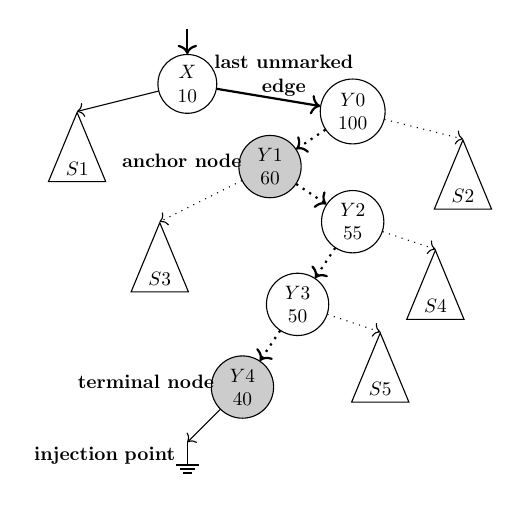
\begin{tikzpicture}[scale=0.7, transform shape]
	\newcommand\XA{0}
\newcommand\YA{0}
\node (x)		[treenode] 									at (\XA,\YA)       						{$X$ \\ 10};
\node (S1)	[subtree] 									at ([shift=({-2,-0.5})]x)  		{ $S1$};
\node (y0)	[treenode] 									at ([shift=({3,-0.5})]x) 			{$Y0$ \\ 100};
\node (y1)	[treenode,fill=black!20]		at ([shift=({-1.5,-1})]y0)		{$Y1$ \\ 60}; 
\node (S2)	[subtree] 									at ([shift=({2,-0.5})]y0)   	{$S2$};
\node (S3)	[subtree] 									at ([shift=({-2,-1})]y1)  		{$S3$};
\node (y2)	[treenode]									at ([shift=({1.5,-1})]y1)			{$Y2$ \\ 55}; 
\node (y3)	[treenode]									at ([shift=({-1,-1.5})]y2)		{$Y3$ \\ 50}; 
\node (S4)	[subtree] 									at ([shift=({1.5,-0.5})]y2)  	{$S4$};
\node (y4)	[treenode,fill=black!20]		at ([shift=({-1,-1.5})]y3)		{$Y4$ \\ 40};
\node (S5)	[subtree] 									at ([shift=({1.5,-0.5})]y3)  	{$S5$}; 
\node (gnd)	[ground] 										at ([shift=({-1,-1})]y4)			{}; 
\node (y1l) [] 													at (\XA-0.10,\YA-1.4) 				{\textbf{anchor node}};
\node (y4l) [] 													at (\XA-0.75,\YA-5.4) 				{\textbf{terminal node}};
\node (x1) 	[rectangle,align=center,minimum size=1cm] at(\XA+1.75,\YA+0.15) 	{\textbf{last unmarked} \\ \textbf{edge}};
\node (x1) 	[rectangle,align=center,minimum size=1cm]at (\XA-1.5,\YA-6.75) 	{\textbf{injection} \textbf{point}};

\path[every node/.style={font=\sffamily\large}]
(\XA,\YA+1) 	edge[->,thick] 		node 					{} (x)
(x) 		edge[->,thick]					node 					{} (y0)
(x) 		edge[->,thin]						node 					{} (S1.north)
(y0) 		edge[->,dotted,thick]		node 					{} (y1)
(y0) 		edge[->,dotted,thin]		node 					{} (S2.north)
(y1) 		edge[->,dotted,thin]		node 					{} (S3.north)
(y1) 		edge[->,dotted,thick]		node 					{} (y2)
(y2) 		edge[->,dotted,thick]		node 					{} (y3)
(y2) 		edge[->,dotted,thin]		node 					{} (S4.north)
(y3) 		edge[->,dotted,thick]		node 					{} (y4)
(y3) 		edge[->,dotted,thin]		node 					{} (S5.north)
(y4) 		edge[->]								node 				 	{} (gnd);



	\end{tikzpicture}
}
\end{minipage}
\end{figure}
\newcommand\XA{0}
\newcommand\YA{0}
\node (x)		[treenode] 									at (\XA,\YA)       						{$X$ \\ 10};
\node (S1)	[subtree] 									at ([shift=({-2,-0.5})]x)  		{ $S1$};
\node (y0)	[treenode] 									at ([shift=({3,-0.5})]x) 			{$Y0$ \\ 100};
\node (y1)	[treenode,fill=black!20]		at ([shift=({-1.5,-1})]y0)		{$Y1$ \\ 60}; 
\node (S2)	[subtree] 									at ([shift=({2,-0.5})]y0)   	{$S2$};
\node (S3)	[subtree] 									at ([shift=({-2,-1})]y1)  		{$S3$};
\node (y2)	[treenode]									at ([shift=({1.5,-1})]y1)			{$Y2$ \\ 55}; 
\node (y3)	[treenode]									at ([shift=({-1,-1.5})]y2)		{$Y3$ \\ 50}; 
\node (S4)	[subtree] 									at ([shift=({1.5,-0.5})]y2)  	{$S4$};
\node (y4)	[treenode,fill=black!20]		at ([shift=({-1,-1.5})]y3)		{$Y4$ \\ 40};
\node (S5)	[subtree] 									at ([shift=({1.5,-0.5})]y3)  	{$S5$}; 
\node (gnd)	[ground] 										at ([shift=({-1,-1})]y4)			{}; 
\node (y1l) [] 													at (\XA-0.10,\YA-1.4) 				{\textbf{anchor node}};
\node (y4l) [] 													at (\XA-0.75,\YA-5.4) 				{\textbf{terminal node}};
\node (x1) 	[rectangle,align=center,minimum size=1cm] at(\XA+1.75,\YA+0.15) 	{\textbf{last unmarked} \\ \textbf{edge}};
\node (x1) 	[rectangle,align=center,minimum size=1cm]at (\XA-1.5,\YA-6.75) 	{\textbf{injection} \textbf{point}};

\path[every node/.style={font=\sffamily\large}]
(\XA,\YA+1) 	edge[->,thick] 		node 					{} (x)
(x) 		edge[->,thick]					node 					{} (y0)
(x) 		edge[->,thin]						node 					{} (S1.north)
(y0) 		edge[->,dotted,thick]		node 					{} (y1)
(y0) 		edge[->,dotted,thin]		node 					{} (S2.north)
(y1) 		edge[->,dotted,thin]		node 					{} (S3.north)
(y1) 		edge[->,dotted,thick]		node 					{} (y2)
(y2) 		edge[->,dotted,thick]		node 					{} (y3)
(y2) 		edge[->,dotted,thin]		node 					{} (S4.north)
(y3) 		edge[->,dotted,thick]		node 					{} (y4)
(y3) 		edge[->,dotted,thin]		node 					{} (S5.north)
(y4) 		edge[->]								node 				 	{} (gnd);



\input{pseudocode/search}
A seek operation keeps track of the node in the \accesspath \space at which the last "right turn" was taken (i.e., right edge was followed). Let us call this node as \anchorNode. Upon reaching the last node, it compares the stored key with the target key. If they do not match, then it is possible that the key may have moved up in the tree. So key stored in the \anchorNode \space is checked to see if has changed. If the key has changed then the seek operation restarts. If the key has not changed, then the key stored in the \anchorNode \space is checked to see if it is undergoing deletion (by checking if its left child edge is marked). If the key is not undergoing deletion, then the seek operation terminates. If the key is undergoing deletion, then it checks if the \anchorNode \space of the current traversal matches with the \anchorNode \space of the previous traversal. If they match, then the seek operation terminates by returning the results of the previous traversal; otherwise it restarts.\par
In the case of insert operation, the seek operation also returns the injection point which is the current contents of the child location at which the insert will occur.

\subsubsection{Execution Phase of an Insert Operation} \paragraph{}
\input{pseudocode/insert}
In the execution phase, an insert operation creates a new node containing the target key. It then adds the new node to the tree at the injection point using a CAS instruction. If the CAS succeeds, then (the new node becomes a part of the tree and) the operation terminates; otherwise, the operation determines if it failed because of a conflicting delete operation in progress. If there is no conflicting delete operation in progress then the operation restarts from the seek phase; otherwise it performs helping (which will be described later) and then restarts from the seek phase.

\subsubsection{Execution Phase of a Delete Operation} \paragraph{}
\begin{figure}[t]
\centering
\caption{An illustration of a simple delete operation. \label{fig:simple}}
{
	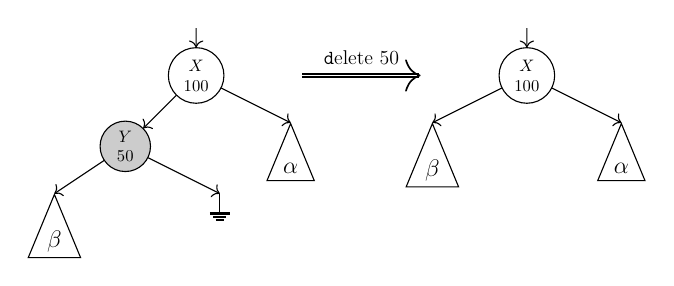
\begin{tikzpicture}[scale=0.6, transform shape]
	\node (a)[treenode] 								at (-3,0)       {$X$ \\ 100};
\node (b)[treenode, fill=black!20] 	at (-4.5,-1.5) 	{$Y$ \\ 50};
\node (c)[subtree] 									at (-1,-1)      {\Large $\alpha$};
\node (d)[subtree] 									at (-6,-2.5)    {\Large $\beta$};
\node (e)[ground] 									at (-2.5,-2.5)	{}; 

\draw[->] (-3, 1) -- (a);
\draw[->] (a) 		-- (b);
\draw[->] (a) 		-- (c.north);
\draw[->] (b) 		-- (d.north);
\draw[->] (b) 		-- (e);


\draw[->, semithick, double] (-0.75, 0) -- node[above, outer sep=3pt] {\large \texttt delete 50} (1.75, 0);

\node (ia)[treenode] 								at (4,0) 				{$X$ \\ 100};
\node (ib)[subtree] 								at (2,-1) 			{\Large $\beta$};
\node (ir)[subtree] 								at (6,-1) 			{\Large $\alpha$};

\draw[->] (4, 1) 	-- (ia);
\draw[->] (ia) 		-- (ib.north);
\draw[->] (ia) 		-- (ir.north);


	\end{tikzpicture}
}
\end{figure}
\begin{figure}[t]
\centering
\caption{An illustration of a complex delete operation. \label{fig:complex}}
{
	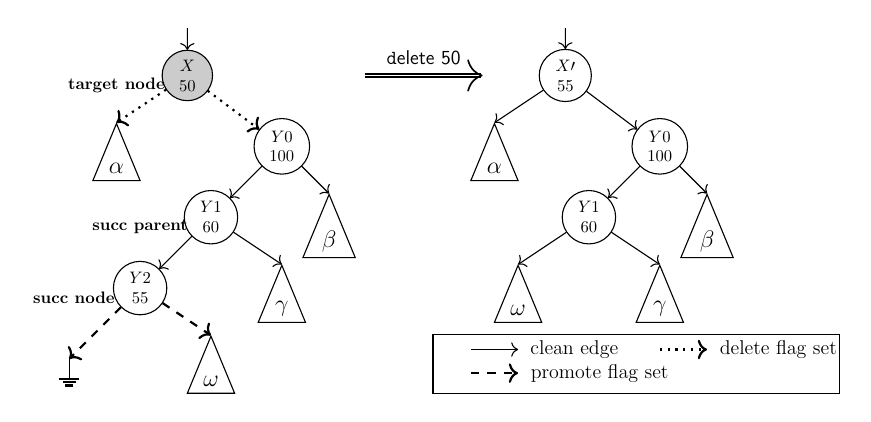
\begin{tikzpicture}[scale=0.6, transform shape]
	\node (x)		[treenode, fill=black!20] 	at (-6,0)       {$X$ \\ 50};
\node (a)		[subtree] 									at (-7.5,-1)  	{\Large $\alpha$};
\node (y0)	[treenode] 									at (-4,-1.5) 		{$Y0$ \\ 100};
\node (y1)	[treenode]									at (-5.5,-3)		{$Y1$ \\ 60}; 
\node (b)		[subtree] 									at (-3,-2.5)    {\Large $\beta$};
\node (y2)	[treenode]									at (-7,-4.5)		{$Y2$ \\ 55}; 
\node (g)		[subtree] 									at (-4,-4)   		{\Large $\gamma$};
\node (gnd)	[ground] 										at (-8.5,-6)		{}; 
\node (o)		[subtree] 									at (-5.5,-5.5)  {\Large $\omega$};
\node (x1) 	[] 													at(-7.5,-0.2) 	{\textbf{target node}};
\node (y1l) [] 													at(-7,-3.2) 		{\textbf{succ parent}};
\node (y2l) [] 													at(-8.4,-4.7) 	{\textbf{succ node}};

\path[every node/.style={font=\sffamily\large}]
%(-8.5, -0.2)edge[->] 								node [above, outer sep=3pt]					{target node} (-6.7,-0.2)
%(-9.5, -4.7)edge[->] 								node [above, outer sep=3pt]					{succ node} (-7.7,-4.7)
(-6, 1) edge[->] 								node 					{} (x)
(x) 		edge[->,dotted,thick] 	node 					{} (y0)
(x) 		edge[->,dotted,thick]		node 					{} (a.north)
(y0) 		edge[->] 								node 					{} (y1)
(y0) 		edge[->] 								node 					{} (b.north)
(y1) 		edge[->] 								node 					{} (y2)
(y1) 		edge[->] 								node 					{} (g.north)
(y2) 		edge[->,dashed,thick]		node 					{} (gnd)
(y2) 		edge[->,dashed,thick]		node 					{} (o.north);

\path[every node/.style={font=\sffamily\small}]
(-2.25, 0) edge[->,semithick, double] node [above, outer sep=3pt] {\large \texttt delete 50} (0.25, 0);

\node (ix)	[treenode] 									at (2,0)       	{$X$$\prime$ \\ 55};
\node (ia)	[subtree] 									at (0.5,-1)  		{\Large $\alpha$};
\node (iy0)	[treenode] 									at (4,-1.5) 		{$Y0$ \\ 100};
\node (iy1)	[treenode]									at (2.5,-3)			{$Y1$ \\ 60}; 
\node (ib)	[subtree] 									at (5,-2.5)    	{\Large $\beta$};
\node (io)	[subtree]										at (1,-4)				{\Large $\omega$}; 
\node (ignd)[subtree] 									at (4,-4)   		{\Large $\gamma$};

\path[every node/.style={font=\sffamily\small}]
(2, 1) 	edge[->] 								node 					{} (ix)
(ix) 		edge[->] 								node 					{} (iy0)
(ix) 		edge[->] 								node 					{} (ia.north)
(iy0) 	edge[->] 								node 					{} (iy1)
(iy0) 	edge[->] 								node 					{} (ib.north)
(iy1) 	edge[->] 								node 					{} (io.north)
(iy1) 	edge[->] 								node 					{} (ignd.north);

%% legend
\draw[->] (0, -5.8) -- (1, -5.8) node[right] {\large ~clean edge};
\draw[->,dotted,thick] (4, -5.8) -- (5, -5.8) node[right] {\large ~delete flag set};
\draw[->,dashed,thick] (0, -6.3) -- (1, -6.3) node[right] {\large ~promote flag set};
\node [thin, draw=black, align=center, minimum width=8.6cm, minimum height=1.25cm] at (3.5, -6.1) {};

	\end{tikzpicture}
}
\end{figure}
The execution of a delete operation starts in the \textit{injection} mode. Once the operation has been injected into the tree, then it advances to the \textit{cleanup} mode.
\begin{figure}[t]
\centering
\caption{An illustration of a simple delete operation. \label{fig:simple}}
{
	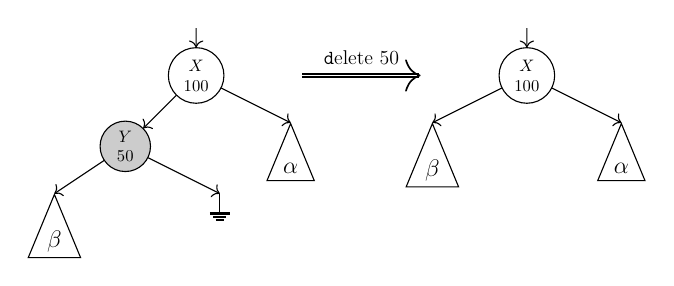
\begin{tikzpicture}[scale=0.6, transform shape]
	\node (a)[treenode] 								at (-3,0)       {$X$ \\ 100};
\node (b)[treenode, fill=black!20] 	at (-4.5,-1.5) 	{$Y$ \\ 50};
\node (c)[subtree] 									at (-1,-1)      {\Large $\alpha$};
\node (d)[subtree] 									at (-6,-2.5)    {\Large $\beta$};
\node (e)[ground] 									at (-2.5,-2.5)	{}; 

\draw[->] (-3, 1) -- (a);
\draw[->] (a) 		-- (b);
\draw[->] (a) 		-- (c.north);
\draw[->] (b) 		-- (d.north);
\draw[->] (b) 		-- (e);


\draw[->, semithick, double] (-0.75, 0) -- node[above, outer sep=3pt] {\large \texttt delete 50} (1.75, 0);

\node (ia)[treenode] 								at (4,0) 				{$X$ \\ 100};
\node (ib)[subtree] 								at (2,-1) 			{\Large $\beta$};
\node (ir)[subtree] 								at (6,-1) 			{\Large $\alpha$};

\draw[->] (4, 1) 	-- (ia);
\draw[->] (ia) 		-- (ib.north);
\draw[->] (ia) 		-- (ir.north);


	\end{tikzpicture}
}
\end{figure}
\begin{figure}[t]
\centering
\caption{An illustration of a complex delete operation. \label{fig:complex}}
{
	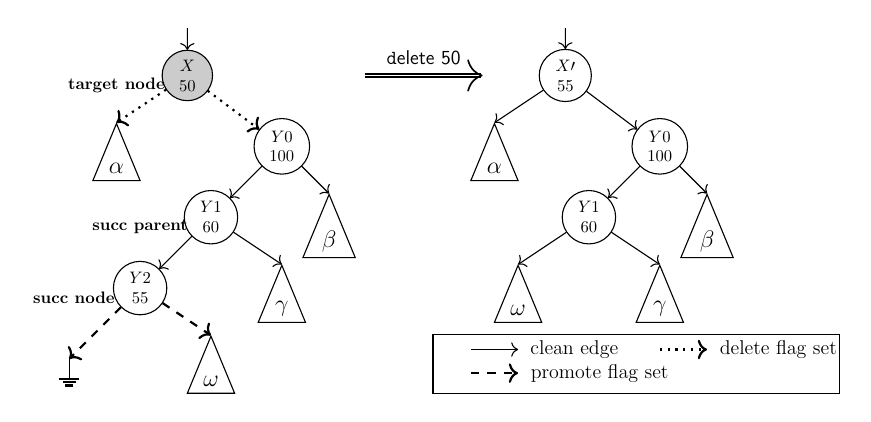
\begin{tikzpicture}[scale=0.6, transform shape]
	\node (x)		[treenode, fill=black!20] 	at (-6,0)       {$X$ \\ 50};
\node (a)		[subtree] 									at (-7.5,-1)  	{\Large $\alpha$};
\node (y0)	[treenode] 									at (-4,-1.5) 		{$Y0$ \\ 100};
\node (y1)	[treenode]									at (-5.5,-3)		{$Y1$ \\ 60}; 
\node (b)		[subtree] 									at (-3,-2.5)    {\Large $\beta$};
\node (y2)	[treenode]									at (-7,-4.5)		{$Y2$ \\ 55}; 
\node (g)		[subtree] 									at (-4,-4)   		{\Large $\gamma$};
\node (gnd)	[ground] 										at (-8.5,-6)		{}; 
\node (o)		[subtree] 									at (-5.5,-5.5)  {\Large $\omega$};
\node (x1) 	[] 													at(-7.5,-0.2) 	{\textbf{target node}};
\node (y1l) [] 													at(-7,-3.2) 		{\textbf{succ parent}};
\node (y2l) [] 													at(-8.4,-4.7) 	{\textbf{succ node}};

\path[every node/.style={font=\sffamily\large}]
%(-8.5, -0.2)edge[->] 								node [above, outer sep=3pt]					{target node} (-6.7,-0.2)
%(-9.5, -4.7)edge[->] 								node [above, outer sep=3pt]					{succ node} (-7.7,-4.7)
(-6, 1) edge[->] 								node 					{} (x)
(x) 		edge[->,dotted,thick] 	node 					{} (y0)
(x) 		edge[->,dotted,thick]		node 					{} (a.north)
(y0) 		edge[->] 								node 					{} (y1)
(y0) 		edge[->] 								node 					{} (b.north)
(y1) 		edge[->] 								node 					{} (y2)
(y1) 		edge[->] 								node 					{} (g.north)
(y2) 		edge[->,dashed,thick]		node 					{} (gnd)
(y2) 		edge[->,dashed,thick]		node 					{} (o.north);

\path[every node/.style={font=\sffamily\small}]
(-2.25, 0) edge[->,semithick, double] node [above, outer sep=3pt] {\large \texttt delete 50} (0.25, 0);

\node (ix)	[treenode] 									at (2,0)       	{$X$$\prime$ \\ 55};
\node (ia)	[subtree] 									at (0.5,-1)  		{\Large $\alpha$};
\node (iy0)	[treenode] 									at (4,-1.5) 		{$Y0$ \\ 100};
\node (iy1)	[treenode]									at (2.5,-3)			{$Y1$ \\ 60}; 
\node (ib)	[subtree] 									at (5,-2.5)    	{\Large $\beta$};
\node (io)	[subtree]										at (1,-4)				{\Large $\omega$}; 
\node (ignd)[subtree] 									at (4,-4)   		{\Large $\gamma$};

\path[every node/.style={font=\sffamily\small}]
(2, 1) 	edge[->] 								node 					{} (ix)
(ix) 		edge[->] 								node 					{} (iy0)
(ix) 		edge[->] 								node 					{} (ia.north)
(iy0) 	edge[->] 								node 					{} (iy1)
(iy0) 	edge[->] 								node 					{} (ib.north)
(iy1) 	edge[->] 								node 					{} (io.north)
(iy1) 	edge[->] 								node 					{} (ignd.north);

%% legend
\draw[->] (0, -5.8) -- (1, -5.8) node[right] {\large ~clean edge};
\draw[->,dotted,thick] (4, -5.8) -- (5, -5.8) node[right] {\large ~delete flag set};
\draw[->,dashed,thick] (0, -6.3) -- (1, -6.3) node[right] {\large ~promote flag set};
\node [thin, draw=black, align=center, minimum width=8.6cm, minimum height=1.25cm] at (3.5, -6.1) {};

	\end{tikzpicture}
}
\end{figure}
\subsubsection{Injection Mode:} In the \textit{injection} mode, the delete operation marks the left child edge of the target node using a CAS instruction. If the CAS instruction succeeds, then the delete operation has been injected into the tree and is guaranteed to complete. Then the operation moves on to the \textit{cleanup} mode. But if the CAS instruction fails, the operation performs helping and restarts from the seek phase (and stays in the \textit{injection} mode).
\input{pseudocode/inject}
\subsubsection{Cleanup Mode:} In the \textit{cleanup} mode, the operation begins by marking the right child edge of the target node using a BTS (Bit Test and Set) instruction (this can also be done using a CAS instruction as well). Note that we maintain an invariant that edges which are once marked cannot be unmarked. Eventually the node is either removed from the tree (by \textit{simple} delete) or replaced with a "new" node containing the next largest key (by \textit{complex} delete). Further, a marked edge is changed only under a specific situation by a delete operation as part of helping (described later). \par
\input{pseudocode/cleanup}
After marking both the edges, an operation checks whether the node is a binary node or not. If it is a binary node, then the delete operation is classified as a \textit{complex} delete; otherwise it is classified as a \textit{simple} delete. Let $T$ be the \terminalnode, $T.parent$ be its parent node and $T.left$ and $T.right$ be the left and right child node respectively, of $T$. We now discuss the two types of delete operation.
\subsubsection{Simple Delete:}
	In this case, either $T.left$ or $T.right$ is a null node. Note that both $T.left$ and $T.right$ may be null nodes in which case $T$ will be a leaf node. Without loss of generality, assume that $T.right$ is a null node. Delete operation attempts to change the pointer at $T.parent$ that is pointing to $T$ to point to $T.left$ using a CAS instruction. If the CAS instruction succeeds, then the operation terminates; otherwise, the delete operation performs another seek operation. If the seek operation either fails to find the target key or returns a \terminalnode \space different from $T$, then $T$ has been already removed from the tree (by another operation as part of helping) and the operation terminates; otherwise, it attempts to remove $T$ from the tree again. Note that the new seek operation may return a different parent node. This process may be repeated multiple times.
\input{pseudocode/findAndMarkSuccessor}
\input{pseudocode/removeSuccessor}
\subsubsection{Complex Delete:} In this case, both $T.left$ and $T.right$ are non-null nodes. The operation now performs the following steps:
\begin{enumerate}
\item Locate the next largest key in the tree, which is the smallest key in the subtree rooted at the right child of the \terminalnode \space $T$. We refer to this key as the \textit{successor key} and the node storing this key as the \textit{successor node}. Let $S$ denote the \textit{successor node} and $S.parent$ denote its parent node.
\item Claim the \textit{successor node}. This involves marking both the child edges of $S$. Note that the left edge of $S$ will be null. To distinguish between marking a \terminalnode \space (for deletion) and marking a \textit{successor node} (for promotion), we steal two bits from the address and refer to them as \deleteFlag \space and \promoteFlag \space respectively. The left edge of $S$ is marked (i.e., \promoteFlag \space is set) using a CAS instruction. As part of marking the left edge, we also store the address of the \terminalnode \space $T$ in the left edge. This is done to enable helping in case the \textit{successor node} is obstructing the progress of another operation. In case if the CAS instruction fails, the operation repeats from step 1. The right edge of $S$ is marked using a BTS instruction.
\item Promote the \textit{successor key}. The \textit{successor key} is copied into the \terminalnode. At the same time, the mark bit in the key is set to indicate that the key currently stored in the \terminalnode \space is the \textit{successor key} and not the target key.
\item The \textit{successor node} $S$ is deleted by changing the pointer at $S.parent$ that is pointing to $S$ to point to the right child of $S$ using a CAS instruction. If the CAS instruction fails, then the operation performs helping if needed. It then finds the \textit{successor node} again by performing a traversal starting from the right child of the \terminalnode \space $T$ and repeats step 4. If the \textit{successor node} is not found in the traversal, then it has been already removed from the tree ( by another operation as part of helping) and the operation moves to step 5. 
\item Note that, at this point, the original key in the \terminalnode \space has been replaced with the \textit{successor key}. Further, its key as well as both its edges are marked. The \terminalnode \space is now replaced with a new node whose contents are same as that of the \terminalnode \space expect that all the fields are unmarked. The \terminalnode \space is then replaced with a new node using a CAS instruction at the parent node. If the CAS instruction succeeds, then the operation terminates; otherwise, as in the case of \textit{simple} delete, it performs another seek operation, this time looking for the \textit{successor key}. If the seek operation either fails to find the \textit{successor key} or returns a \terminalnode \space different from $T$, then $T$ has been already replaced (by another operation as part of helping) and the operation terminates. On the other hand if the seek operation finds the \terminalnode \space $T$ with the \textit{successor key}, it attempts to replace $T$ again. Note that the new seek operation may return a different parent node. This process may be repeated multiple times.
\end{enumerate}
\input{pseudocode/findSmallest}
\input{pseudocode/updateModeAndType}
\subsubsection{Helping} \paragraph{}
To enable helping, whenever traversing the tree to locate either a target key or a \textit{successor key}, we keep track of the last unmarked edge encountered in the traversal. Whenever an operation fails while executing a CAS instruction, it helps the operation in progress at the child end of the unmarked edge if different from its own operation. Note that, when traversing the tree looking for a target key, the last unmarked edge will always be found because of the sentinel keys. However, when traversing the tree looking for a \textit{successor key}, the last unmarked edge may not always exist since the traversal starts from the middle of the tree from the right child of a \terminalnode. Recall that $T$ denotes a \terminalnode \space and $T.right$ its right child node. If no unmarked edge is found during the traversal from $T.right$, then helping is performed along the edge ($T$,$T.right$),that is, the delete operation in progress at $T.right$ is helped. This will involve modifying the edge ($T$,$T.right$) even though the edge is marked to either remove $T.right$ (if \textit{simple} delete) or replace $T.right$ with a fresh node (if \textit{complex} delete).

\section{Experimental Evaluation}
\subsubsection{Experimental Setup:} We conducted our experiments on an X86\_64 AMD Opteron 6276 machine running GNU/Linux operating system. We used gcc 4.6.3 compiler with optimization flag set to $O3$. The Table I shows the hardware features of this machine. All implementations were written in C++. To compare the performance of different implementations, we considered the following parameters:
\begin{enumerate}
\item \textbf{Maximum Tree Size:} This depends on the size of the key space. We consider five different key ranges: 1000(1K), 10,000 (10K), 100,000 (100K), 1 million (1M) and 10 million (10M) keys. To capture only the steady state behaviour we \textit{pre-populated} the tree to 50$\%$ of its maximum size, prior to starting the simulation run.
\item \textbf{Relative Distribution of Various Operations:} We consider three different workload  distributions: (a) \textit{read-dominated} workload : 90$\%$ search, 9$\%$ insert and 1$\%$ delete, (b) \textit{mixed} workload : 70$\%$ search, 20$\%$ insert and 10$\%$ delete and (c) \textit{write-dominated} workload : 0$\%$ search, 50$\%$ insert and 50$\%$ delete
\item \textbf{Maximum Degree of Contention:} This depends on number of threads concurrently operating on the tree. We varied the number of threads from 1 to 128 in increments in powers of 2.
\end{enumerate}
\begin{table}[h]
\caption{hardware features}
\begin{tabular}{|l|l|}
\hline
CPU packages      & 4         \\ \hline
Cores per package & 8         \\ \hline
Threads per core  & 2         \\ \hline
Clock frequency   & 2.3 GHz   \\ \hline
L1 cache (I/D)    & 64KB/16KB \\ \hline
L2 cache          & 2 MB      \\ \hline
L3 cache          & 6 MB      \\ \hline
Memory            & 256 GB    \\ \hline
\end{tabular}
\quad
\begin{tabular}{|c|c|c|c|c|}
\hline
\multirow{2}{*}{\textbf{Algorithm}} & \multicolumn{2}{c|}{\textbf{\begin{tabular}[c]{@{}c@{}}\# of \\ Objects\\  Allocated\end{tabular}}} & \multicolumn{2}{c|}{\textbf{\begin{tabular}[c]{@{}c@{}}\#of Atomic \\ Instructions\\  Executed\end{tabular}}} \\ \cline{2-5} 
                                    & \textbf{Ins}                                     & \textbf{Del}                                     & \textbf{Ins}                                          & \textbf{Del}                                          \\ \hline
\textbf{Ellen \& \textit{et al}.}                      & 4                                                & 2                                                & 3                                                     & 4                                                     \\ \hline
\textbf{Howley \& Jones}                     & 2                                                & 1                                                & 3                                                     & upto 9                                                \\ \hline
\textbf{Natarajan \& Mittal}        & 2                                                & 0                                                & 1                                                     & 3                                                     \\ \hline
\textbf{This work}                  & 1                                                & 1                                                & 1                                                     & upto 6                                                \\ \hline
\end{tabular}
\end{table}
We compared the performance of different implementations with respect to two metrics:
\begin{enumerate}
	\item \textbf{System Throughput:} it is defined as the number of operations executed per unit time.
	\item \textbf{Avg Seek Length:} it is defined as the average length of the access path of a seek operation.
\end{enumerate}
\newpage
\begin{tikzpicture}
	\begin{groupplot}[group style={group size= 2 by 4},height=5cm,width=6.4cm]
		\nextgroupplot[title=Read-Dominated,ylabel={keyrange: 1K},symbolic x coords={1,2,4,8,16,32,64,128},xtick=data]
				\addplot[red,mark=triangle] 	table{Data/HJ-BST.dat}; \label{plots:HJ-BST}
				\addplot[blue,mark=asterisk] 	table{Data/NM-BST.dat}; \label{plots:NM-BST}
				\addplot[green,mark=square] 	table{Data/RM-BST.dat}; \label{plots:RM-BST}
				\coordinate (top) at (rel axis cs:0,1);% coordinate at top of the first plot
		\nextgroupplot[title=Mixed,symbolic x coords={1,2,4,8,16,32,64,128},xtick=data]
				\addplot[red,mark=triangle] 	table{Data/HJ-BST.dat};
				\addplot[blue,mark=asterisk] 	table{Data/NM-BST.dat};
				\addplot[green,mark=square] 	table{Data/RM-BST.dat};
		\nextgroupplot[ylabel={keyrange: 10K},symbolic x coords={1,2,4,8,16,32,64,128},xtick=data]
				\addplot[red,mark=triangle] 	table{Data/HJ-BST.dat};
				\addplot[blue,mark=asterisk] 	table{Data/NM-BST.dat};
				\addplot[green,mark=square] 	table{Data/RM-BST.dat};
		\nextgroupplot[symbolic x coords={1,2,4,8,16,32,64,128},xtick=data]
				\addplot[red,mark=triangle] 	table{Data/HJ-BST.dat};
				\addplot[blue,mark=asterisk] 	table{Data/NM-BST.dat};
				\addplot[green,mark=square] 	table{Data/RM-BST.dat};
		\nextgroupplot[ylabel={keyrange: 100K},symbolic x coords={1,2,4,8,16,32,64,128},xtick=data]
				\addplot[red,mark=triangle] 	table{Data/HJ-BST.dat};
				\addplot[blue,mark=asterisk] 	table{Data/NM-BST.dat};
				\addplot[green,mark=square] 	table{Data/RM-BST.dat};
		\nextgroupplot[symbolic x coords={1,2,4,8,16,32,64,128},xtick=data]
				\addplot[red,mark=triangle] 	table{Data/HJ-BST.dat};
				\addplot[blue,mark=asterisk] 	table{Data/NM-BST.dat};
				\addplot[green,mark=square] 	table{Data/RM-BST.dat};
		\nextgroupplot[xlabel={Number of Threads},ylabel={keyrange: 1M},symbolic x coords={1,2,4,8,16,32,64,128},xtick=data]
				\addplot[red,mark=triangle] 	table{Data/HJ-BST.dat};
				\addplot[blue,mark=asterisk] 	table{Data/NM-BST.dat};
				\addplot[green,mark=square] 	table{Data/RM-BST.dat};
		\nextgroupplot[xlabel={Number of Threads},symbolic x coords={1,2,4,8,16,32,64,128},xtick=data]
				\addplot[red,mark=triangle] 	table{Data/HJ-BST.dat};
				\addplot[blue,mark=asterisk] 	table{Data/NM-BST.dat};
				\addplot[green,mark=square] 	table{Data/RM-BST.dat};
				\coordinate (bot) at (rel axis cs:0,0);% coordinate at bottom of the last plot
	\end{groupplot}
	\path (top-|current bounding box.west)-- node[anchor=south,rotate=90] {Throughput (million ops/sec)} (bot-|current bounding box.west);
	\path (top|-current bounding box.north)-- coordinate(legendpos) (bot|-current bounding box.north);
	\matrix[matrix of nodes, anchor=south, draw, inner sep=0.2em, draw] at ([yshift=1ex]legendpos)
  {
    \ref{plots:HJ-BST}& HJ-BST&[5pt]
    \ref{plots:NM-BST}& NM-BST&[5pt]
    \ref{plots:RM-BST}& RM-BST\\
	};
\end{tikzpicture}
\newpage
\begin{tikzpicture}
	\begin{groupplot}[group style={group size= 1 by 4},height=5cm,width=6.4cm]
		\nextgroupplot[title=Write-Dominated,ylabel={keyrange: 1K},symbolic x coords={1,2,4,8,16,32,64,128},xtick=data]
				\addplot[red,mark=triangle] 	table{Data/HJ-BST.dat}; 
				\addplot[blue,mark=asterisk] 	table{Data/NM-BST.dat}; 
				\addplot[green,mark=square] 	table{Data/RM-BST.dat}; 
				\coordinate (top) at (rel axis cs:0,1);% coordinate at top of the first plot
		\nextgroupplot[ylabel={keyrange: 10K},symbolic x coords={1,2,4,8,16,32,64,128},xtick=data]
				\addplot[red,mark=triangle] 	table{Data/HJ-BST.dat};
				\addplot[blue,mark=asterisk] 	table{Data/NM-BST.dat};
				\addplot[green,mark=square] 	table{Data/RM-BST.dat};
		\nextgroupplot[ylabel={keyrange: 100K},symbolic x coords={1,2,4,8,16,32,64,128},xtick=data]
				\addplot[red,mark=triangle] 	table{Data/HJ-BST.dat};
				\addplot[blue,mark=asterisk] 	table{Data/NM-BST.dat};
				\addplot[green,mark=square] 	table{Data/RM-BST.dat};
		\nextgroupplot[xlabel={Number of Threads},ylabel={keyrange: 1M},symbolic x coords={1,2,4,8,16,32,64,128},xtick=data]
				\addplot[red,mark=triangle] 	table{Data/HJ-BST.dat};
				\addplot[blue,mark=asterisk] 	table{Data/NM-BST.dat};
				\addplot[green,mark=square] 	table{Data/RM-BST.dat};
				\coordinate (bot) at (rel axis cs:0,0);% coordinate at bottom of the last plot
	\end{groupplot}
	\path (top-|current bounding box.west)-- node[anchor=south,rotate=90] {Throughput (million ops/sec)} (bot-|current bounding box.west);
	\path (top|-current bounding box.north)-- coordinate(legendpos) (bot|-current bounding box.north);
	\matrix[matrix of nodes, anchor=south, draw, inner sep=0.2em, draw] at ([yshift=1ex]legendpos)
  {
    \ref{plots:HJ-BST}& HJ-BST&[5pt]
    \ref{plots:NM-BST}& NM-BST&[5pt]
    \ref{plots:RM-BST}& RM-BST\\
	};
\end{tikzpicture}

\input{discussion}

\bibliographystyle{splncs03}
\bibliography{Bibliography/citations}

\end{document}